\documentclass[tikz,border=10pt]{standalone}
\usepackage{amsmath,amssymb}
\begin{document}
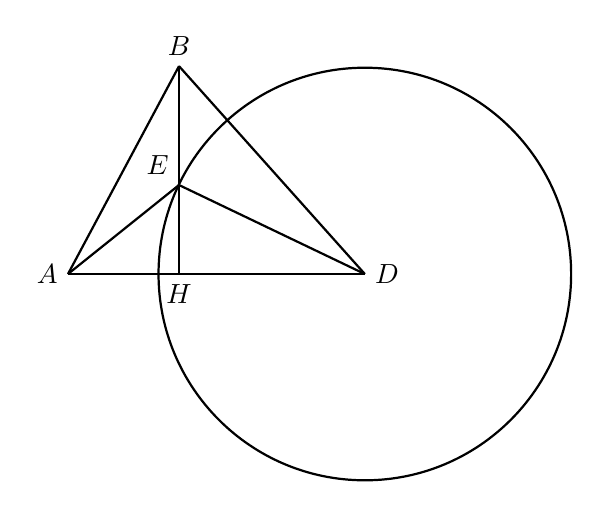
\begin{tikzpicture}[scale=1, line width=0.8pt]
  \coordinate (A) at (0,0);
  \coordinate (H) at (1.41,0);
  \coordinate (D) at (3.77,0);
  \coordinate (B) at (1.41,2.64);
  \coordinate (E) at (1.41,1.13);

  \draw (A) -- (B);
  \draw (B) -- (D);
  \draw (A) -- (D);
  \draw (B) -- (H);
  \draw (A) -- (E);
  \draw (E) -- (D);
  \draw (D) circle (2.62);

  \node[above] at (B) {$B$};
  \node[above left] at (E) {$E$};
  \node[left] at (A) {$A$};
  \node[below] at (H) {$H$};
  \node[right] at (D) {$D$};
\end{tikzpicture}
\end{document}
